%%%%%%%%%%%%%%%%%%%%%%%%%%%%%%%%%%%%%%%%%
% Short Sectioned Assignment
% LaTeX Template
% Version 1.0 (5/5/12)
%
% This template has been downloaded from:
% http://www.LaTeXTemplates.com
%
% Original author:
% Frits Wenneker (http://www.howtotex.com)
%
% License:
% CC BY-NC-SA 3.0 (http://creativecommons.org/licenses/by-nc-sa/3.0/)
%
%%%%%%%%%%%%%%%%%%%%%%%%%%%%%%%%%%%%%%%%%

%----------------------------------------------------------------------------------------
%	PACKAGES AND OTHER DOCUMENT CONFIGURATIONS
%----------------------------------------------------------------------------------------

\documentclass[letterpaper, 11pt]{scrartcl} % Letter paper and 11pt font size
\usepackage[letterpaper]{geometry}

\usepackage[T1]{fontenc} % Use 8-bit encoding that has 256 glyphs
%\usepackage{fourier} % Use the Adobe Utopia font for the document - comment this line to return to the LaTeX default
\usepackage{libertine}
\usepackage[english]{babel} % English language/hyphenation
\usepackage{amsmath,amsfonts,amsthm} % Math packages

\usepackage{lipsum} % Used for inserting dummy 'Lorem ipsum' text into the template

\usepackage{sectsty} % Allows customizing section commands
\usepackage{hyperref}
\usepackage{url}
\usepackage{tikz}
\usetikzlibrary{arrows}
\usepackage{multirow}
\urlstyle{same} % Make URL use the same font as the surroundings.
\allsectionsfont{\centering \normalfont\scshape} % Make all sections centered, the default font and small caps

\usepackage{fancyhdr} % Custom headers and footers
\pagestyle{fancyplain} % Makes all pages in the document conform to the custom headers and footers
\fancyhead{} % No page header - if you want one, create it in the same way as the footers below
\fancyfoot[L]{} % Empty left footer
\fancyfoot[C]{} % Empty center footer
\fancyfoot[R]{\thepage} % Page numbering for right footer
\renewcommand{\headrulewidth}{0pt} % Remove header underlines
\renewcommand{\footrulewidth}{0pt} % Remove footer underlines
\setlength{\headheight}{13.6pt} % Customize the height of the header

\numberwithin{equation}{section} % Number equations within sections (i.e. 1.1, 1.2, 2.1, 2.2 instead of 1, 2, 3, 4)
\numberwithin{figure}{section} % Number figures within sections (i.e. 1.1, 1.2, 2.1, 2.2 instead of 1, 2, 3, 4)
\numberwithin{table}{section} % Number tables within sections (i.e. 1.1, 1.2, 2.1, 2.2 instead of 1, 2, 3, 4)

\setlength\parindent{0pt} % Removes all indentation from paragraphs - comment this line for an assignment with lots of text

%----------------------------------------------------------------------------------------
%	TITLE SECTION
%----------------------------------------------------------------------------------------

\newcommand{\horrule}[1]{\rule{\linewidth}{#1}} % Create horizontal rule command with 1 argument of height

\title{	
\normalfont \normalsize 
%\textsc{University of Houston} \\ [25pt] % Your university, school and/or department name(s)
\horrule{0.5pt} \\[0.4cm] % Thin top horizontal rule
\huge Proposal for Unifying the Coordinate Systems Used by Different Reconstruction Algorithms for Muon Study \\ % The assignment title
\horrule{2pt} \\[0.5cm] % Thick bottom horizontal rule
}

\author{Shih-Kai Lin} % Your name

\date{\normalsize\today} % Today's date or a custom date

\begin{document}

\maketitle % Print the title

%----------------------------------------------------------------------------------------
%	SECTION 1
%----------------------------------------------------------------------------------------

\section{Motivation}

Event reconstruction usually involves point or track reconstruction. The coordinate of a point or the direction of a track depends on the reference frame it refers to. Each detector has its own most convenient and intuitive coordinate system, namely, the local coordinate system of the detector. For example, each AD has its local coordinate system with the origin at the center of the mineral oil detector volume and $x$ and $y$ axis parallel to the experimental hall the AD is in. Similarly, the water pool has its local coordinate system with the origin at the center of the outer water pool detector volume and $x$ and $y$ axis parallel to the experimental hall. Naturally we refer the position of an IBD event to the AD local coordinate system. However we can also refer it to the water pool local coordinate system. By doing so we get a new set of numerical values which is related to the old set by a translation and possibly a rotation. For point-like events there is no reason to adopt any coordinate system other than that of the detector designed for that kind of events. However, muons could leave multiple traces in different detectors, and a common coordinate system across the detectors is required to reconstruct the spacial information. In data, a muon is identified as a group of triggers satisfying prescribed timing and energy conditions. If a muon triggers multiple detector subsystems, different spacial reconstruction algorithms which refer to their own local coordinate systems will be invoked, resulting in inconsistent spacial information. More importantly, if one wants to study the spacial correlation between a muon and its induced events, a common coordinate system is a necessity.

%------------------------------------------------

\section{Goal}

In this proposal we propose to add to each event a reconstructed point referring to the global coordinate system alongside its local coordinate in order to facilitate muon studies. In case there are difficulties to include one additional spacial reconstruction information, this document could serve as a reference of coordinate transformation between different coordinate systems.

%------------------------------------------------

\section{Muon Tagging}

Since one single muon could go through multiple detectors, a muon is practically identified as a group of triggers scattered in the data satisfying prescribed timing and energy requirements. Tagging muons is nontrivial and is detailed in \cite{jjling+hqlu}. In this document ``muon" refers to the officially tagged muon events in the production files.

%------------------------------------------------

\section{Coordinate Systems}

Daya Bay has three halls, 8 ADs and muon systems. Naturally adopting a coordinate system which respects the symmetry and orientation of the individual detector can greatly simply the analysis. However there still exists a coordinate system common to all halls and detectors called global coordinate system whose origin is that of hall 4, $x$ points to the East and $y$ points to the North. For more information, see \cite{coordsys}. To transform the global coordinate of a point to its local coordinate, one simply has to do a translation followed by a rotation,
\begin{equation}
\vec{r}_l=O_{lg}(\vec{r}_g-\vec{r}_{gl})
\end{equation}
where $\vec{r}_l$ and $\vec{r}_g$ are the local and global coordinates, respectively, $\vec{r}_{gl}$ is the vector from the origin of the global to that of the local coordinate and $O_{lg}$ is the \emph{active} rotation matrix to align the axes of the local with those of the global coordinate system. See Fig.~\ref{fig:Fig1}. For more detailed figures, see \cite{bob}.

\begin{figure}
\centering
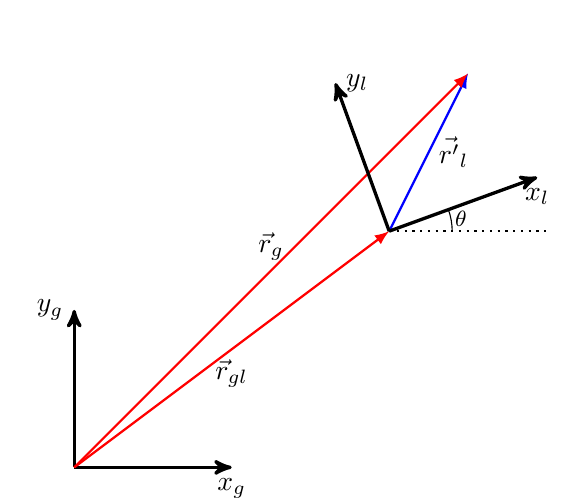
\begin{tikzpicture}[
    scale=2,
    axis/.style={very thick, ->, >=stealth'},
    important line/.style={thick},
    dashed line/.style={dashed, thin},
    pile/.style={thick, ->, >=stealth', shorten <=2pt, shorten
    >=2pt},
    every node/.style={color=black}
    ]
    % axis
    \draw[axis] (0,0)  -- (1,0) node(xline)[below] {$x_g$};
    \draw[axis] (0,0) -- (0,1) node(yline)[left] {$y_g$};
    \draw[red, thick, ->, >=latex] (0,0) -- (2,1.5) node[midway,below] {$\vec{r}_{gl}$};
    \draw[blue, thick, ->, >=latex] (2,1.5) -- (2.5,2.5) node[midway,right] {$\vec{r'}_{l}$};
    \draw[red, thick, ->, >=latex] (0,0) -- (2.5,2.5) node[midway,above] {$\vec{r}_{g}$};
    \draw[axis] (2,1.5) -- +(20:1) node[below] {$x_l$};
    \draw[axis] (2,1.5) -- +(110:1) node[right] {$y_l$};
    \draw[black, thick, dotted] (2,1.5) -- (3,1.5);
    \draw (2.4,1.5) arc (0:20:0.4);
    \node at (2.455,1.578) {\footnotesize $\theta$};
\end{tikzpicture}
\caption{relationship between global and local coordinate systems} \label{fig:Fig1}
\end{figure}

Note that the $z$ axes of the global and local coordinate systems are parallel, therefore the rotation matrix $O_{lg}$ is a single parameter matrix,
\begin{equation}
	O_{lg}=
	\begin{pmatrix}
	\cos\theta & \sin\theta & 0 \\
  -\sin\theta & \cos\theta & 0  \\
  0 & 0  & 1
	\end{pmatrix}
\end{equation}
Since the axes of different local coordinate systems in the same hall are parallel, detectors in the same hall share the same rotation angle $\theta$. Table~\ref{table:rotationangle} lists the rotation angles read out from NuWa.

\begin{table}
	\centering
	\begin{tabular}{|c|c|c|c|}
		\hline
		& hall 1 & hall 2 & hall 3 \\
		\hline
		$\theta$ (degree) & -122.90 & 79.71 & 150.55 \\
		\hline
	\end{tabular}
	\caption{the \emph{active} rotation angle for each hall from global to local coordinate system}
	\label{table:rotationangle}
\end{table}

As for the translation vector $\vec{r}_{gl}$, Table~\ref{table:translation} lists the components with respect to the global coordinate system.% Not every detector is listed and this will be explained in the following section.

\begin{table}
	\centering
	\begin{tabular}{|c|c|c c c|}
		\hline
		hall & detector & $x$ (mm) & $y$ (mm) & $z$ (mm)\\
		\hline
		\multirow{5}{*}{1} & AD1 & -18079.5 & -799699 & -7092.5 \\
		& AD2 & -14960.5 & -804521 & -7092.5 \\
		& IWS & -16520 & -802110 & -6564 \\
		& OWS & -16520 & -802110 & -7066 \\
		& RPC & -17458.1 & -799739 & 5390 \\
		\hline
		\multirow{5}{*}{2} & AD1 & 472323 & 60325.2 & -3712.5 \\
		& AD2 & 471297 & 65974.8 & -3712.5 \\
		& IWS & 471810 & 63150 & -3184 \\
		& OWS & 471810 & 63150 & -3686 \\
		& RPC & 471765 & 60600.9 & 8770 \\
		\hline
		\multirow{7}{*}{3} & AD1 & -406758 & 812082 & -2242.5 \\
		& AD2 & -411758 & 809258 & -2242.5 \\
		& AD3 & -409582 & 817082 & -2242.5 \\
		& AD4 & -414582 & 814258 & -2242.5 \\
		& IWS & -410670 & 813170 & -1714 \\
		& OWS & -410670 & 813170 & -2216 \\
		& RPC & -415344 & 809957 & 10240 \\
		\hline
	\end{tabular}
	\caption{the components of the translation vector $\vec{r}_{gl}$ with respect to the global coordinate system}
	\label{table:translation}
\end{table}

The transformation formula for a direction vector from global to local coordinate is
\begin{equation}
  \vec{v}_l=O_{lg}\vec{v}_g
\end{equation}
where $\vec{v}_l$ and $\vec{v}_g$ are the local and global coordinates, respectively.

To transform a coordinate from local to global, one simply does an inverse transformation,
\begin{equation}
	\vec{r}_g=O_{lg}^{-1}\vec{r}_l+\vec{r}_{gl}
\end{equation}
\begin{equation}
	\vec{v}_g=O_{lg}^{-1}\vec{v}_l
\end{equation}

%----------------------------------------------------------------------------------------

\section{Coordinate Systems and Units Adopted by Algorithms}

In P14A production data, under \texttt{\footnotesize{/Event/Rec/}} there are 7 reconstruction algorithms, 3 for AD, 1 for water pool, 1 for RPC and 2 for muon track. There is also one algorithm under \texttt{\footnotesize{\path{/Event/Data/Physics/}}} for muon track reconstruction. Each algorithm has its own coordinate system and some even use different unit from the others. Table~\ref{table:algdetail} shows the purpose of and coordinate and unit used by each algorithm.
\begin{table}
	\small
	\centering
	\begin{tabular}{|c|c|c|c|c|}
		\hline
		path & algorithm & purpose & coordinate & unit \\
		\hline
		\multirow{7}{*}{\texttt{\scriptsize{/Event/Rec/}}} & AdScaled & AD point recon. & AD local & mm \\
		\cline{2-5}
		& AdSimple & AD point recon. & AD local & mm \\
		\cline{2-5}
		& AdTime   & AD point recon. & AD local & mm \\
		\cline{2-5}
		& AdUnfold & AD muon track recon. & AD local & mm \\
		\cline{2-5}
		& MuonCombined & AD muon track recon. & AD local & mm \\
		\cline{2-5}
		& PoolSimple & water pool muon point recon. & OWS local & \textcolor{red}{m} \\
		\cline{2-5}
		& RpcSimple & RPC muon point recon. & OWS local & mm \\
		\hline
		\texttt{\scriptsize{/Event/Data/Physics/}} & MuonRecSimple & pool+RPC muon track recon. & OWS local & \textcolor{red}{m} \\
		\hline
	\end{tabular}
	\caption{details of reconstruction algorithms}
	\label{table:algdetail}
\end{table}

%----------------------------------------------------------------------------------------

\section{Discussion}

Owing to the engagement of the AD muon reconstruction algorithms \texttt{\footnotesize{AdUnfold}} and \texttt{\footnotesize{MuonCombined}}, which put a muon and its induced events on the same footing, the needs for using a common coordinate system are greatly reduced. However if one wants to study the spacial correlation of induced events by non-AD muons, one still has to resort to a common coordinate system. Besides, muon flux depends on mountain profile which is only manifested using global coordinate system. To conclude this proposal, the advantages and disadvantages of having global coordinate information are listed.\newline

Advantage:
\begin{itemize}
	\item be able to study spacial correlation between a non-AD muon and its induced events
	\item be able to study muon flux as a function of the mountain profile
\end{itemize}

Disadvantage:
\begin{itemize}
	\item additional disk space
	\item each algorithm needs modification
\end{itemize}

%----------------------------------------------------------------------------------------

\bibliographystyle{unsrt}
\bibliography{references}

\end{document}